% -*- TeX -*-
\documentclass[aspectratio=169]{beamer}

\title{PyLith v3.0 Tutorial}
\subtitle{Quasi-static Simulations with No Fault}
\author{Charles Williams \\
  Brad Aagaard \\
  Matthew Knepley}
\institute{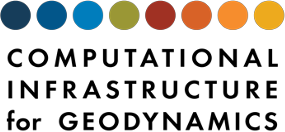
\includegraphics[scale=1.5]{../../logos/cig_logo_dots}%
  \hspace{4em}%
\raisebox{1em}{\includegraphics[scale=1.0]{../../logos/cig_short_pylith}}}
\date{June 20, 2022}


% ---------------------------------------------------- CUSTOMIZATION
\usetheme{CIG}
% Style information for PyLith presentations.

% Colors
\definecolor{ltorange}{rgb}{1.0, 0.74, 0.41} % 255/188/105
\definecolor{orange}{rgb}{0.96, 0.50, 0.0} % 246/127/0

\definecolor{ltred}{rgb}{1.0, 0.25, 0.25} % 255/64/64
\definecolor{red}{rgb}{0.79, 0.00, 0.01} % 201/0/3

\definecolor{ltpurple}{rgb}{0.81, 0.57, 1.00} % 206/145/255
\definecolor{purple}{rgb}{0.38, 0.00, 0.68} % 97/1/175

\definecolor{ltblue}{rgb}{0.2, 0.73, 1.0} % 51/187/255
\definecolor{mdblue}{rgb}{0.28, 0.50, 0.80} % 72/128/205
\definecolor{blue}{rgb}{0.12, 0.43, 0.59} % 30/110/150

\definecolor{ltltgreen}{rgb}{0.7, 1.00, 0.7} % 96/204/14
\definecolor{ltgreen}{rgb}{0.37, 0.80, 0.05} % 96/204/14
\definecolor{green}{rgb}{0.23, 0.49, 0.03} % 59/125/8
  
\definecolor{dkslate}{rgb}{0.18, 0.21, 0.28} % 47/53/72
\definecolor{mdslate}{rgb}{0.45, 0.50, 0.68} % 114/127/173
\definecolor{ltslate}{rgb}{0.85, 0.88, 0.95} % 216/225/229


\newcommand{\includefigure}[2][]{{\centering\includegraphics[#1]{#2}\par}}
\newcommand{\highlight}[1]{{\bf\usebeamercolor[fg]{structure}#1}}
\newcommand{\important}[1]{{\color{red}#1}}
\newcommand{\issue}[2]{\item[Issue:] {\color{red}#1}\\{\item[Soln:] \color{blue}#2}\\[4pt]}

\setbeamercolor{alerted text}{fg=ltgreen}
\setbeamertemplate{description item}[align left]


\newcommand{\lhs}[1]{{\color{blue}#1}}
\newcommand{\rhs}[1]{{\color{red}#1}}
\newcommand{\annotateL}[2]{%
  {\color{blue}\underbrace{\color{blue}#1}_{\color{blue}\mathclap{#2}}}}
\newcommand{\annotateR}[2]{%
  {\color{red}\underbrace{\color{red}#1}_{\color{red}\mathclap{#2}}}}
\newcommand{\eqnannotate}[2]{%
  {\color{blue}%
  \underbrace{\color{black}#1}_{\color{blue}\mathclap{#2}}}}

\newcommand{\trialvec}[1][]{{\vec{\psi}_\mathit{trial}^{#1}}}
\newcommand{\trialscalar}[1][]{{\psi_\mathit{trial}^{#1}}}
\newcommand{\basisvec}[1][]{{\vec{\psi}_\mathit{basis}^{#1}}}
\newcommand{\basisscalar}[1][]{{\psi_\mathit{basis}^{#1}}}

\newcommand{\tensor}[1]{\bm{#1}}
\DeclareMathOperator{\Tr}{Tr}

\usefonttheme[onlymath]{serif}

% minted shortcuts
\newminted{cfg}{bgcolor=ltslate,autogobble,fontsize=\tiny}
\newminted{bash}{bgcolor=ltltgreen,autogobble,fontsize=\tiny}

% PyLith components
\newcommand{\pylith}[1]{{\ttfamily\color{magenta}#1}}



% ========================================================= DOCUMENT
\begin{document}

% ------------------------------------------------------------ SLIDE
\maketitle

\logo{\includegraphics[height=4.5ex]{../../logos/cig_short_pylith}}

% ========================================================== SECTION
\section{{\ttfamily examples/box-2d}}

% ========================================================== SUBSECTION
\subsection{Overview}

% ------------------------------------------------------------ SLIDE
\begin{frame}
  \frametitle{Axial and Shear Deformation of a 2D Box: {\ttfamily examples/box-2d}}
  \summary{}

  \includefigure[height=6.1cm]{figs/geometry}

  \vfill
  Solve the static and quasistatic boundary elasticity equation in a 2D box with uniform material properties.
  
\end{frame}


% ------------------------------------------------------------ SLIDE
\begin{frame}
  \frametitle{Steps in example}
  \summary{}

  \begin{description}
    \item[Step 1] \highlight{Axial extension with Dirichlet (displacement) boundary conditions}
    \item[Step 2] \highlight{Shear deformation with Dirichlet (displacement) boundary conditions}
    \item[Step 3] \highlight{Shear deformation with Dirichlet (displacement) and Neumann (traction) boundary conditions}
    \item[Step 4] Same as Step 2 but with initial conditions equal to the analytical solution
    \item[Step 5] Shear deformation with time-dependent Dirichlet (displacement) and Neumann (traction) boundary conditions
  \end{description}
  
\end{frame}


% ------------------------------------------------------------ SLIDE
\begin{frame}
  \frametitle{Concepts covered}
  \summary{}

  \begin{itemize}
  \item Ingredients for a PyLith simulation
  \item PyLith \pylith{MeshIOAscii} mesh format
  \item PyLith \pylith{.cfg} paremeter files
  \item \pylith{ZeroDB}, \pylith{UniformDB}, and \pylith{SimpleDB} spatial databases
  \item Dirichlet (displacement) boundary conditions
  \item Neumann (traction) boundary conditions
  \item Running a simulation
  \item Visualization of simulation results using Paraview
  \end{itemize}

\end{frame}


% ------------------------------------------------------------ SLIDE
\begin{frame}
  \frametitle{Overview of a PyLith simulation}
  \summary{}

  \includefigure[height=7.0cm]{figs/pylith_simulation}
  
\end{frame}


% ========================================================== SUBSECTION
\subsection{Finite-Element Mesh}

% ------------------------------------------------------------ SLIDE
\begin{frame}
  \frametitle{Geometry}
  \summary{}

  \includefigure[height=7.0cm]{figs/geometry}
  
\end{frame}


% ------------------------------------------------------------ SLIDE
\begin{frame}
  \frametitle{Creating the finite-element mesh}
  \summary{For this very simple example, we create the mesh by hand}

  \includefigure[height=6.5cm]{figs/mesh}
  
\end{frame}


% ------------------------------------------------------------ SLIDE
\begin{frame}
  \frametitle{Files used in simulations}
  \summary{Files are in directory {\ttfamily examples/box-2d}}

  \begin{description}
  \item[README.md] Brief description of the various examples
  \item[*.cfg] PyLith parameter files
  \item[*.mesh] Finite-element mesh file generated manually using a text editor
  \item[*.spatialdb] Spatial database files
  \item[viz] Directory containing ParaView Python scripts and other files for visualizing results
  \item[output] Directory containing simulation output; created automatically when running the simulations
  \end{description}

\end{frame}
  

% ========================================================== SECTION
\subsection{step01-axialdisp}

% ------------------------------------------------------------ SLIDE
\begin{frame}
  \frametitle{Step 1: Overview}
  \summary{Axial extension in the x direction}

  \includefigure[height=6.5cm]{figs/step01-diagram}
      
\end{frame}


% ------------------------------------------------------------ SLIDE
\begin{frame}
  \frametitle{Step 1: Physics}
  \summary{}

  \begin{minipage}{0.35\textwidth}
    {\scriptsize
    \begin{gather*}
      \vec{s} = \left(\begin{array}{c} \vec{u} \end{array}\right)^T \\
      \boldsymbol{\nabla} \cdot \boldsymbol{\sigma}(\vec{u}) = \vec{0} \\
      u_x = -u_0 \text{ on boundary\_xneg} \\
      u_x = +u_0 \text{ on boundary\_xpos} \\
      u_y = 0 \text{ on boundary\_yneg}
    \end{gather*}}
  \end{minipage}
  \hfill
  \begin{minipage}{0.55\textwidth}
    \includefigure[height=6.5cm]{figs/step01-diagram}
  \end{minipage}
      
\end{frame}


% ------------------------------------------------------------ SLIDE
\begin{frame}[t,fragile]
  \frametitle{Step 1: Physics to simulation parameters}
  \summary{}

  \begin{minipage}[t]{0.35\textwidth}
    {\scriptsize
    \begin{gather*}
      \vec{s} = \left(\begin{array}{c} \vec{u} \end{array}\right)^T \tikzmark{solution1}\\
      \boldsymbol{\nabla} \cdot \boldsymbol{\sigma}(\vec{u}) = \vec{0} \tikzmark{material1}\\
      u_x = -u_0 \text{ on boundary\_xneg} \tikzmark{bc1}\\
      u_x = +u_0 \text{ on boundary\_xpos} \\
      u_y = 0 \text{ on boundary\_yneg}
    \end{gather*}}
  \end{minipage}
  \hfill
  \begin{minipage}[t]{0.60\textwidth}
    % Solution
    \begin{onlyenv}<2>
      \tikzmark{solution1-cfg}
      \begin{cfgcode}
        # These are the defaults; not included in pylithapp.cfg.
        [pylithapp.problem]
        solution = pylith.problems.SolnDisp
        
        [pylithapp.problem.solution.subfields]
        displacement.basis_order = 1
      \end{cfgcode}
    \end{onlyenv}
    %
    % Governing equations
    \begin{onlyenv}<3>
      \tikzmark{material1-cfg}
      \begin{cfgcode}
        # These are the defaults; not included in pylithapp.cfg.
        [pylithapp.problem]
        materials = [elastic]
        materials.elastic = pylith.materials.Elasticity

        [pylithapp.problem.materials.elastic]
        elastic.bulk_rheology = pylith.materials.IsotropicLinearElasticity
      \end{cfgcode}
    \end{onlyenv}
    %
    % Boundary conditions
    \begin{onlyenv}<4>
      \tikzmark{bc1-cfg}
      \begin{cfgcode}
        [pylithapp.problem]
        bc = [bc_xneg, bc_xpos, bc_yneg]
        bc.bc_xneg = pylith.bc.DirichletTimeDependent
        bc.bc_xpos = pylith.bc.DirichletTimeDependent
        bc.bc_yneg = pylith.bc.DirichletTimeDependent
        
        [pylithapp.problem.bc.bc_xpos]
        constrained_dof = [0]
        label = boundary_xpos
        ...
      \end{cfgcode}
    \end{onlyenv}
  \end{minipage}

    
  \begin{tikzpicture}[overlay,remember picture]
    \draw[physics-arrow,visible on=<2>] ($(pic cs:solution1-cfg)-(0,2em)$) to (pic cs:solution1);
    \draw[physics-arrow,visible on=<3>] ($(pic cs:material1-cfg)-(0,2em)$) to (pic cs:material1);
    \draw[physics-arrow,visible on=<4>] ($(pic cs:bc1-cfg)-(0,2em)$) to (pic cs:bc1);
  \end{tikzpicture}

  
\end{frame}


% ------------------------------------------------------------ SLIDE
\begin{frame}
  \frametitle{Step 1: Input files}
  \summary{}

  \begin{description}
  \item[quad.mesh] Finite-element mesh as a text file
  \item[pylithapp.cfg] PyLith parameter file common to all steps
  \item[step01\_axialdisp.cfg] PyLith parameter file
  \end{description}
    
\end{frame}


% ------------------------------------------------------------ SLIDE
\begin{frame}[fragile]
  \frametitle{Step 1: Run the simulation}
  \summary{}

\begin{bashcode}
pylith step01_axialdisp.cfg

# Output
 >> /software/unix/py39-venv/pylith-debug/lib/python3.9/site-packages/pylith/meshio/MeshIOObj.py:44:read
 -- meshioascii(info)
 -- Reading finite-element mesh
 >> /src/cig/pylith/libsrc/pylith/meshio/MeshIO.cc:94:void pylith::meshio::MeshIO::read(topology::Mesh *)
 -- meshioascii(info)
 -- Component 'reader': Domain bounding box:
    (-6000, 6000)
    (-16000, -0)

# -- many lines omitted --

 -- Solving problem.
0 TS dt 0.01 time 0.
    0 SNES Function norm 1.245882095312e-02 
    Linear solve converged due to CONVERGED_ATOL iterations 1
    1 SNES Function norm 6.738354969624e-18 
  Nonlinear solve converged due to CONVERGED_FNORM_ABS iterations 1
1 TS dt 0.01 time 0.01
 >> /software/unix/py39-venv/pylith-debug/lib/python3.9/site-packages/pylith/problems/Problem.py:201:finalize
 -- timedependent(info)
 -- Finalizing problem.
\end{bashcode}
  
\end{frame}


% ------------------------------------------------------------ SLIDE
\begin{frame}
  \frametitle{Step 1: Visualize results}
  \summary{Run the {\tt viz/plot\_dispwarp.py} Python script from within ParaView}

  \includefigure[height=7.0cm]{figs/step01-solution}
    
\end{frame}


% ========================================================== SECTION
\subsection{step02-sheardisp}

% ------------------------------------------------------------ SLIDE
\begin{frame}
  \frametitle{Step 2: Overview}
  \summary{Simple shear deformation using Dirichlet (displacement) boundary conditions}

  \includefigure[height=6.5cm]{figs/step02-diagram}
      
\end{frame}


% ------------------------------------------------------------ SLIDE
\begin{frame}[t]
  \frametitle{Step 2: Physics}
  \summary{}

  \begin{minipage}{0.35\textwidth}
    {\scriptsize
    \begin{gather*}
      \vec{s} = \left(\begin{array}{c} \vec{u} \end{array}\right)^T \\
      \boldsymbol{\nabla} \cdot \boldsymbol{\sigma}(\vec{u}) = \vec{0} \\
      u_x = ax \text{ on boundary\_xneg} \\
      u_x = ax \text{ on boundary\_xpos} \\
      u_y = a(y+8\mathrm{km}) \text{ on boundary\_yneg} \\
      u_y = a(y+8\mathrm{km}) \text{ on boundary\_ypos}
    \end{gather*}}
  \end{minipage}
  \hfill
  \begin{minipage}{0.55\textwidth}
    \includefigure[height=6.5cm]{figs/step02-diagram}
  \end{minipage}
      
\end{frame}


% ------------------------------------------------------------ SLIDE
\begin{frame}[t,fragile]
  \frametitle{Step 2: Physics to simulation parameters}
  \summary{}

  \begin{minipage}[t]{0.35\textwidth}
    {\scriptsize
    \begin{gather*}
      \vec{s} = \left(\begin{array}{c} \vec{u} \end{array}\right)^T \tikzmark{solution2}\\
      \boldsymbol{\nabla} \cdot \boldsymbol{\sigma}(\vec{u}) = \vec{0} \tikzmark{material2}\\
      u_x = ax \text{ on boundary\_xneg} \tikzmark{bc2}\\
      u_x = ax \text{ on boundary\_xpos} \\
      u_y = a(y+8\mathrm{km}) \text{ on boundary\_yneg} \\
      u_y = a(y+8\mathrm{km}) \text{ on boundary\_ypos}
    \end{gather*}}
  \end{minipage}
  \hfill
  \begin{minipage}[t]{0.60\textwidth}
    % Solution
    \begin{onlyenv}<2>
      \tikzmark{solution2-cfg}
      \begin{cfgcode}
        # These are the defaults; not included in pylithapp.cfg.
        [pylithapp.problem]
        solution = pylith.problems.SolnDisp
        
        [pylithapp.problem.solution.subfields]
        displacement.basis_order = 1
      \end{cfgcode}
    \end{onlyenv}
    %
    % Governing equations
    \begin{onlyenv}<3>
      \tikzmark{material2-cfg}
      \begin{cfgcode}
        # These are the defaults; not included in pylithapp.cfg.
        [pylithapp.problem]
        materials = [elastic]
        materials.elastic = pylith.materials.Elasticity

        [pylithapp.problem.materials.elastic]
        elastic.bulk_rheology = pylith.materials.IsotropicLinearElasticity
      \end{cfgcode}
    \end{onlyenv}
    %
    % Boundary conditions
    \begin{onlyenv}<4>
      \tikzmark{bc2-cfg}
      \begin{cfgcode}
        [pylithapp.problem]
        bc = [bc_xneg, bc_yneg, bc_xpos, bc_ypos]
        bc.bc_xneg = pylith.bc.DirichletTimeDependent
        bc.bc_yneg = pylith.bc.DirichletTimeDependent
        bc.bc_xpos = pylith.bc.DirichletTimeDependent
        bc.bc_ypos = pylith.bc.DirichletTimeDependent
        
        [pylithapp.problem.bc.bc_xpos]
        constrained_dof = [1]
        label = boundary_xpos
        ...
      \end{cfgcode}
    \end{onlyenv}
  \end{minipage}

    
  \begin{tikzpicture}[overlay,remember picture]
    \draw[physics-arrow,visible on=<2>] ($(pic cs:solution2-cfg)-(0,2em)$) to (pic cs:solution2);
    \draw[physics-arrow,visible on=<3>] ($(pic cs:material2-cfg)-(0,2em)$) to (pic cs:material2);
    \draw[physics-arrow,visible on=<4>] ($(pic cs:bc2-cfg)-(0,2em)$) to (pic cs:bc2);
  \end{tikzpicture}

  
\end{frame}


% ------------------------------------------------------------ SLIDE
\begin{frame}
  \frametitle{Step 2: Input files}
  \summary{}

  \begin{description}
  \item[quad.mesh] Finite-element mesh as a text file
  \item[pylithapp.cfg] PyLith parameter file common to all steps
  \item[step02\_sheardisp.cfg] PyLith parameter file
  \item[sheardisp\_bc\_xneg.spatialdb] Displacement field on boundary\_xneg
  \item[sheardisp\_bc\_xpos.spatialdb] Displacement field on boundary\_xpos
  \item[sheardisp\_bc\_yneg.spatialdb] Displacement field on boundary\_yneg
  \item[sheardisp\_bc\_ypos.spatialdb] Displacement field on boundary\_ypos
  \end{description}
    
\end{frame}


% ------------------------------------------------------------ SLIDE
\begin{frame}[fragile]
  \frametitle{Step 2: Run the simulation}
  \summary{}

\begin{bashcode}
pylith step02_sheardisp.cfg

# Output
 >> /software/unix/py39-venv/pylith-debug/lib/python3.9/site-packages/pylith/meshio/MeshIOObj.py:44:read
 -- meshioascii(info)
 -- Reading finite-element mesh
 >> /src/cig/pylith/libsrc/pylith/meshio/MeshIO.cc:94:void pylith::meshio::MeshIO::read(topology::Mesh *)
 -- meshioascii(info)
 -- Component 'reader': Domain bounding box:
    (-6000, 6000)
    (-16000, -0)

# -- many lines omitted --

 -- Solving problem.
0 TS dt 0.01 time 0.
    0 SNES Function norm 2.239977678460e-03 
    Linear solve converged due to CONVERGED_ATOL iterations 1
    1 SNES Function norm 1.964321818484e-18 
  Nonlinear solve converged due to CONVERGED_FNORM_ABS iterations 1
1 TS dt 0.01 time 0.01
 >> /software/unix/py39-venv/pylith-debug/lib/python3.9/site-packages/pylith/problems/Problem.py:201:finalize
 -- timedependent(info)
 -- Finalizing problem.
\end{bashcode}
  
\end{frame}


% ------------------------------------------------------------ SLIDE
\begin{frame}
  \frametitle{Step 2: Visualize results}
  \summary{Run the {\tt viz/plot\_dispwarp.py} Python script from within ParaView}

  \includefigure[height=7.0cm]{figs/step02-solution}
    
\end{frame}


% ========================================================== SECTION
\subsection{step03-sheardisptract}

% ------------------------------------------------------------ SLIDE
\begin{frame}
  \frametitle{Step 3: Overview}
  \summary{Simple shear deformation using Dirichlet (displacement) and Neuammn (traction) boundary conditions}

  \includefigure[height=6.5cm]{figs/step03-diagram}
      
\end{frame}


% ------------------------------------------------------------ SLIDE
\begin{frame}[t]
  \frametitle{Step 3: Physics}
  \summary{}

  \begin{minipage}{0.35\textwidth}
    {\scriptsize
    \begin{gather*}
      \vec{s} = \left(\begin{array}{c} \vec{u} \end{array}\right)^T \\
      \boldsymbol{\nabla} \cdot \boldsymbol{\sigma}(\vec{u}) = \vec{0} \\
      \left. \begin{array}{c} u_x = a(y+8\mathrm{km}) \\ u_y = ax \end{array}\right\} \text{ on boundary\_xneg} \\
      \left. \begin{array}{c} u_x = a(y+8\mathrm{km}) \\ u_y = ax \end{array}\right\} \text{ on boundary\_xpos} \\
      \tau_t = -2\mu a \text{ on boundary\_yneg} \\
      \tau_t = -2\mu a \text{ on boundary\_ypos}
    \end{gather*}}
  \end{minipage}
  \hfill
  \begin{minipage}{0.55\textwidth}
    \includefigure[height=6.5cm]{figs/step03-diagram}
  \end{minipage}
      
\end{frame}


% ------------------------------------------------------------ SLIDE
\begin{frame}[t,fragile]
  \frametitle{Step 3: Physics to simulation parameters}
  \summary{}

  \begin{minipage}[t]{0.35\textwidth}
    {\scriptsize
    \begin{gather*}
      \vec{s} = \left(\begin{array}{c} \vec{u} \end{array}\right)^T \tikzmark{solution3}\\
      \boldsymbol{\nabla} \cdot \boldsymbol{\sigma}(\vec{u}) = \vec{0} \tikzmark{material3}\\
      \left. \begin{array}{c} u_x = a(y+8\mathrm{km}) \\ u_y = ax \end{array}\right\} \text{ on boundary\_xneg} \tikzmark{bc3} \\
      \left. \begin{array}{c} u_x = a(y+8\mathrm{km}) \\ u_y = ax \end{array}\right\} \text{ on boundary\_xpos} \\
      \tau_t = -2\mu a \text{ on boundary\_yneg} \\
      \tau_t = -2\mu a \text{ on boundary\_ypos}
    \end{gather*}}
  \end{minipage}
  \hfill
  \begin{minipage}[t]{0.60\textwidth}
    % Solution
    \begin{onlyenv}<2>
      \tikzmark{solution3-cfg}
      \begin{cfgcode}
        # These are the defaults; not included in pylithapp.cfg.
        [pylithapp.problem]
        solution = pylith.problems.SolnDisp
        
        [pylithapp.problem.solution.subfields]
        displacement.basis_order = 1
      \end{cfgcode}
    \end{onlyenv}
    %
    % Governing equations
    \begin{onlyenv}<3>
      \tikzmark{material3-cfg}
      \begin{cfgcode}
        # These are the defaults; not included in pylithapp.cfg.
        [pylithapp.problem]
        materials = [elastic]
        materials.elastic = pylith.materials.Elasticity

        [pylithapp.problem.materials.elastic]
        elastic.bulk_rheology = pylith.materials.IsotropicLinearElasticity
      \end{cfgcode}
    \end{onlyenv}
    %
    % Boundary conditions
    \begin{onlyenv}<4>
      \tikzmark{bc3-cfg}
      \begin{cfgcode}
        [pylithapp.problem]
        bc = [bc_xneg, bc_yneg, bc_xpos, bc_ypos]
        bc.bc_xneg = pylith.bc.DirichletTimeDependent
        bc.bc_xpos = pylith.bc.DirichletTimeDependent
        bc.bc_yneg = pylith.bc.NeumannTimeDependent
        bc.bc_ypos = pylith.bc.NeumannTimeDependent
        
        [pylithapp.problem.bc.bc_xpos]
        constrained_dof = [0, 1]
        label = boundary_xpos
        ...
      \end{cfgcode}
    \end{onlyenv}
  \end{minipage}

    
  \begin{tikzpicture}[overlay,remember picture]
    \draw[physics-arrow,visible on=<2>] ($(pic cs:solution3-cfg)-(0,2em)$) to (pic cs:solution3);
    \draw[physics-arrow,visible on=<3>] ($(pic cs:material3-cfg)-(0,2em)$) to (pic cs:material3);
    \draw[physics-arrow,visible on=<4>] ($(pic cs:bc3-cfg)-(0,2em)$) to (pic cs:bc3);
  \end{tikzpicture}

  
\end{frame}


% ------------------------------------------------------------ SLIDE
\begin{frame}
  \frametitle{Step 3: Input files}
  \summary{}

  \begin{description}
  \item[quad.mesh] Finite-element mesh as a text file
  \item[pylithapp.cfg] PyLith parameter file common to all steps
  \item[step03\_sheardisptract.cfg] PyLith parameter file
  \item[sheardisp\_bc\_xneg.spatialdb] Displacement field on boundary\_xneg
  \item[sheardisp\_bc\_xpos.spatialdb] Displacement field on boundary\_xpos
  \end{description}
    
\end{frame}


% ------------------------------------------------------------ SLIDE
\begin{frame}[fragile]
  \frametitle{Step 3: Run the simulation}
  \summary{}

\begin{bashcode}
pylith step03_sheardisptract.cfg

# Output
 >> /software/unix/py39-venv/pylith-debug/lib/python3.9/site-packages/pylith/meshio/MeshIOObj.py:44:read
 -- meshioascii(info)
 -- Reading finite-element mesh
 >> /src/cig/pylith/libsrc/pylith/meshio/MeshIO.cc:94:void pylith::meshio::MeshIO::read(topology::Mesh *)
 -- meshioascii(info)
 -- Component 'reader': Domain bounding box:
    (-6000, 6000)
    (-16000, -0)

# -- many lines omitted --

 -- Solving problem.
0 TS dt 0.01 time 0.
    0 SNES Function norm 6.059797141590e-03 
    Linear solve converged due to CONVERGED_ATOL iterations 1
    1 SNES Function norm 2.140441363908e-18 
  Nonlinear solve converged due to CONVERGED_FNORM_ABS iterations 1
1 TS dt 0.01 time 0.01
 >> /software/unix/py39-venv/pylith-debug/lib/python3.9/site-packages/pylith/problems/Problem.py:201:finalize
 -- timedependent(info)
 -- Finalizing problem.
\end{bashcode}
  
\end{frame}


% ------------------------------------------------------------ SLIDE
\begin{frame}
  \frametitle{Step 3: Visualize results}
  \summary{Run the {\tt viz/plot\_dispwarp.py} Python script from within ParaView}

  \includefigure[height=7.0cm]{figs/step03-solution}
    
\end{frame}


% ======================================================================
\end{document}


% End of file
